\documentclass{beamer}
\usepackage[italian]{babel}
\usepackage[utf8]{inputenc}

\usetheme{Copenhagen} 
\usecolortheme{crane}

\title[avifauna.fem2ambiente]{Sviluppo e-commerce\\avifauna.fem2ambiente.com}
\author[Mattia Curatitoli]{\textbf{Mattia Curatitoli} \and \\[1cm] 
	Relatore: \textbf{Prof. Daniela Micucci} \and \\
	Correlatore: \textbf{Dr. Emanuele Ferri}}
\date{Ottobre 2015}

% --personal definitions--
\def \unimib {Università degli Studi di Milano Bicocca}
\def \fem {FEM2-Ambiente}
\def \femsrl {FEM2-Ambiente Srl}
\def \zpl {ZooPlantLab}
\def \wp {WordPress}
\def \js {JavaScript}
\def \b {Bootstrap}
\newcommand{\tag}[1] {\small{\texttt{$<$#1$>$}}}
\newcommand{\dja}[1] {\small{\{\% \texttt{#1} \%\}}}
\newcommand{\burl}[1] {\footnotesize{\url{#1}}}

\begin{document}

\begin{frame}
\maketitle
\end{frame}

\begin{frame}
 \begin{center}
  {\huge FEM2 - Ambiente}\\[1cm]
   Uno spin-off del Dipartimento di Biotecnologie e Bioscienze dell'Università degli studi di Milano-Bicocca \\[1cm]
   La mission dell'azienda è creare prodotti e servizi per il largo pubblico finalizzati alla conoscenza e tutela della biodiversità.
 \end{center}
\end{frame}

\begin{frame}
 \frametitle{\fem}
 \begin{center}
  La crescita di {\fem} sul mercato ha portato alla creazione del sito dedicato \url{www.fem2ambiente.com} dove è presente un e-commerce per la vendita di prodotti per l'analisi di acqua ed eco-prodotti per la casa
 \end{center}
\end{frame}


La crescita di {\fem} sul mercato ha portato alla creazione del sito dedicato \url{www.fem2ambiente.com} basato su \emph{Joomla!}, un \emph{CMS} (Content Management System) molto diffuso, utile per la gestione dei contenuti del sito web senza la necessità di avere conoscenze tecniche \cite{joomla}. Ad esso è stata aggiunta l'estensione \emph{VirtueMart}, una soluzione open-source per la gestione dell'e-commerce che ad oggi permette l'acquisto di prodotti per l'analisi di acqua e aria rivolti a privati, imprese e per l'educazione nelle scuole, oltre ad eco-prodotti per la casa e per la cura degli animali \cite{virtuemart}.





\begin{frame}
\frametitle{Accesso programmatico}
\framesubtitle{Modalità di accesso}
\begin{columns}
  \column{0.45\textwidth}
  \begin{center}
  Accesso diretto ai database mySQL pubblici del progetto tramite client SQL 
  \end{center}
  
  \column{0.55\textwidth}
	\begin{figure}
		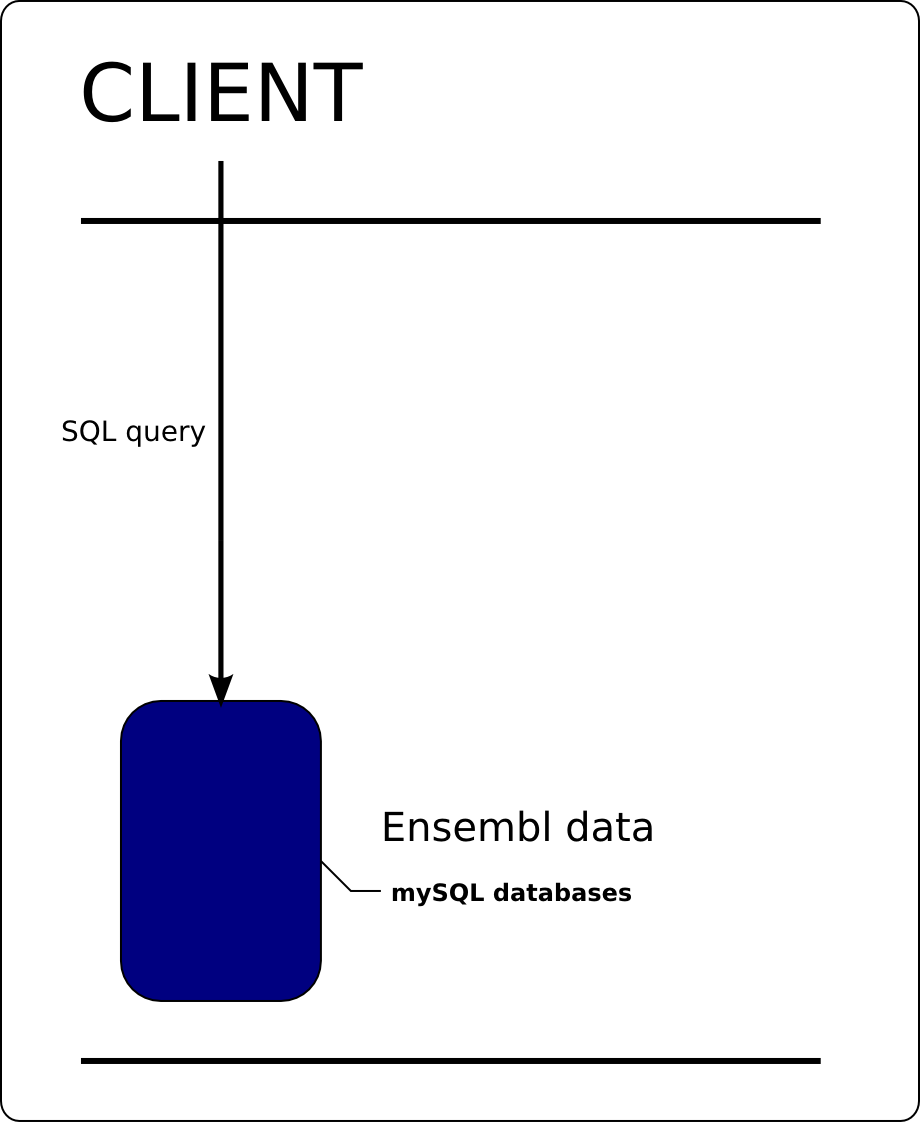
\includegraphics[scale=0.45]{images/mysql.png}
	\end{figure}
\end{columns}
\end{frame}

\begin{frame}
\frametitle{REST API}
\begin{center}
I dati sono organizzati in endpoints,\\ 
l'interrogazione del database avviene via HTTP. \\
La query è codificata nell'URL \\[1cm]
\end{center}
\pause
\texttt{beta.rest.ensembl.org} + \pause \\
\texttt{\hspace{1cm} /taxonomy/id} + \pause \\
\texttt{\hspace{1cm} /Homo sapiens?content-type=application/xml}
\end{frame}


\end{document}
